\section{clemens\_text}\label{clemens_text} %TODO
 
\subsection{Analyse: BART 2.0}

Analysiert wurde \href{http://www.bart-anaphora.org/}{BART} in der Version 2.0, 
wie sie \href{http://www.bart-anaphora.org/release/bart-2.0.tar.gz}{hier} zu finden ist.
Es stehen dem Nutzer zwei Modi zur Nutzung zur Verfügung.
\begin{itemize}
\item BART-WebServer als end-to-end Blackbox Lösung
\item BART-full zum Trainieren eines neuen Modells
\end{itemize}
Erstere erzeugt aus einem Rohtext Input einen Output der Form, 
die in Abb.\ref{bart_webUI_output} zu sehen ist.

\begin{lstlisting}[language=xml]
?xml version="1.0" encoding="UTF-8"?>
<!DOCTYPE words SYSTEM "words.dtd">
<words>
  <word id="word_1">Late</word>
  <word id="word_2">in</word>
  <word id="word_3">the</word>
  <word id="word_4">afternoon</word>
  <word id="word_5">of</word>
  <word id="word_6">a</word>
  <word id="word_7">chilly</word>
  <word id="word_8">day</word>
  <word id="word_9">in</word>
  <word id="word_10">February</word>
  <word id="word_11">,</word>
  ...
  \end{lstlisting}


\begin{figure}[ht]
\begin{center}
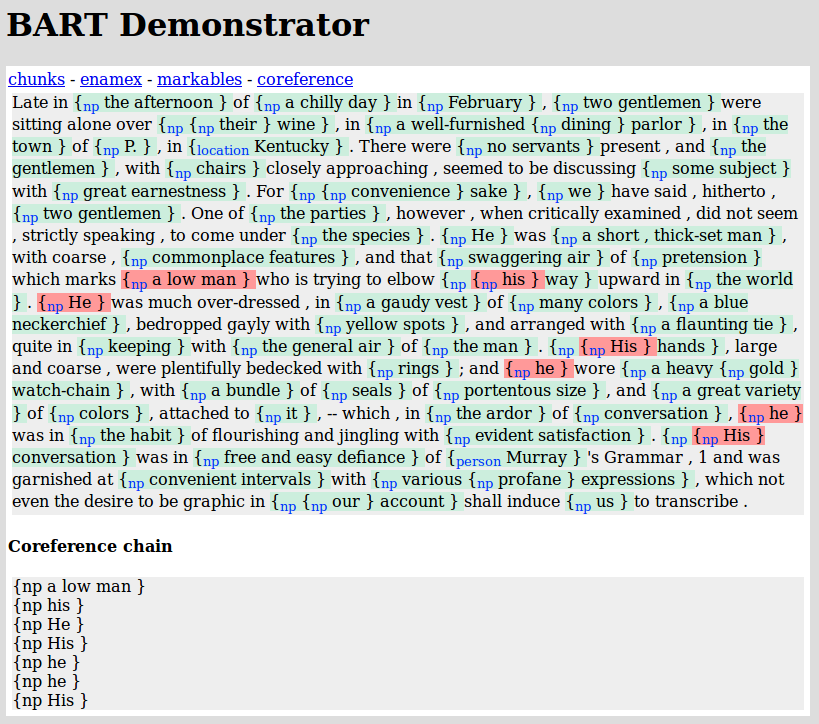
\includegraphics[width=12cm]{./img/cle/bart_webUI_output.png}
 % bart_webUI_output.png: 819x724 pixel, 72dpi, 28.89x25.54 cm, bb=0 0 819 724
\caption{BART 2.0: Output für WebInterface der Blackbox Version}
\label{bart_webUI_output}
\end{center}
\end{figure}



% 
% \begin{itemize}
% \item modulares Toolkit 
% \begin{itemize}
% \item beinhaltet verschiedene Pipelines zur Vorverarbeitung
% \end{itemize}
% \item Input als Reintext oder modifziertes MMAX Format
% \item 2 Modi zur Benutzung
% \item leichte Benutzung, aber schlecht anzupassen
% \end{itemize}



 \subsection{Erstellung BuildIndex} %TODO titel